\chapter{Recursos}

\section{Recursos materiales}
\begin{itemize}
    \item Servidor del CECAD de la Universidad Distrital con las siguientes características:
    \begin{itemize}
        \item Intel Core i7 9th
        \item 8 Gb RAM
        \item 250 GB Almacenamiento
    \end{itemize}
    \item Plataforma en la nube
        \begin{itemize}
        \item Amazon Web Services
        \item Google Cloud Computing Services
        \item Heroku
        \item Microsoft Azure
    \end{itemize}
    \item Sistemas de computo propios
    \item Raspberry Pi 3
\end{itemize}
\section{Recursos humanos}
\begin{itemize}
    \item Profesores directores de grupo y asociados
    \item Profesores de la facultad
    \item Miembros del grupo de investigación
\end{itemize}
\section{Presupuesto total del proyecto}

Para este proyecto los fondos propios son todos aquellos asumidos por los autores del proyecto. Bonos son todos aquellos fondos otorgados por plataformas de servicios en la nube. En la figura \ref{presupuesto} se definen el panorama presupuestal del proyecto.
\begin{figure}[H]
    \centering
    
\includegraphics[width=\linewidth]{secciones/Imagenes/presupuesto.eps}
    \caption{}
    \label{presupuesto}
\end{figure}
En la figura \ref{Bonos} se precisa la procedencia de los bonos.
\begin{figure}[H]
    \centering
    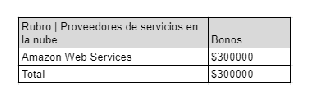
\includegraphics[width=\linewidth]{secciones/Imagenes/Bonos.eps}
    \caption{}
    \label{Bonos}
\end{figure}
En la figura \ref{materiales} se especifican los materiales e insumos requeridos para el desarrollo del proyecto.
\begin{figure}[H]
    \centering
    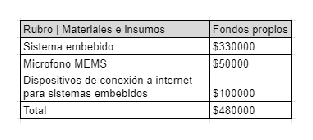
\includegraphics[width=\linewidth]{secciones/Imagenes/Materiales.eps}
    \caption{}
    \label{materiales}
\end{figure}
\newpage
\section{Cronograma}
\begin{figure}[H]
    \centering
    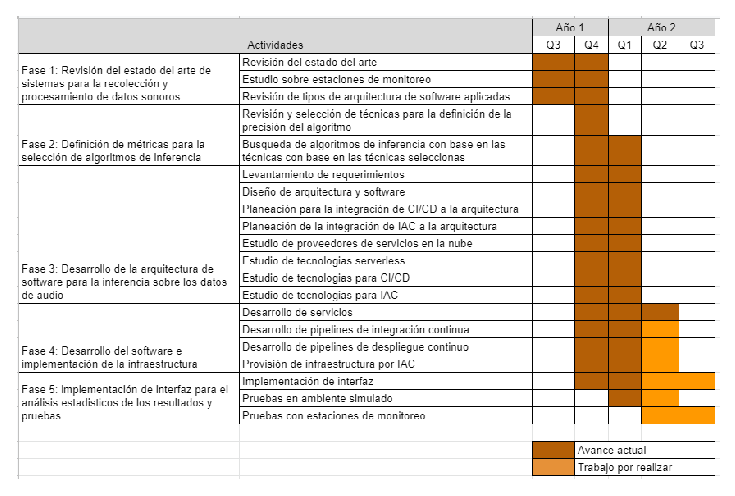
\includegraphics[width=\linewidth]{secciones/Imagenes/cronograma.eps}
    \caption{}
    \label{fig:my_label}
\end{figure}
\newpage